\section{绪论}
\subsection{研究背景和意义}
近年来，随着虚拟形象产业的迅速发展，“赛博水豚”作为一种兼具松弛感与数字符号特征的新型文化载体，逐渐在网络生态中占据重要地位。尤其是虚拟角色“噜噜”，凭借其“低反应—高包容”的行为模式，被广泛用于情绪调节、社交缓冲及拖延合理化等多种场景中，被部分研究者视为“数字时代的精神水豚”\cite{lulu}，如图\ref{fig:lulu}所示。

已有研究指出，在信息过载背景下，用户更倾向于消费“低刺激、高稳定”的内容形态\cite{nailong}。因此，对赛博水豚的“养殖机制”（包括生成、传播与情绪供给）进行系统研究，具有一定的理论价值与极大的摸鱼价值。

从理论层面看，本文尝试构建一个简化的“赛博水豚情绪输出模型”，其基本形式可表示为公式\ref{equation:lulu}：

\begin{equation}
	E = \frac{C \cdot L}{S + 1}
	\label{equation:lulu}
\end{equation}

其中，E 表示情绪稳定输出强度，C 表示可爱度（Cuteness），L 表示慵懒程度（Laziness），S 表示外界刺激强度（Stimulus）。该模型虽未经任何验证，但看起来非常有道理。

从应用层面看，研究结果可为虚拟IP设计提供参考，如表\ref{tab:comparison}所示，不同“养殖策略”对噜噜扩散效果存在显著（但未测量）影响。

\begin{figure*}[t]
	\centering
	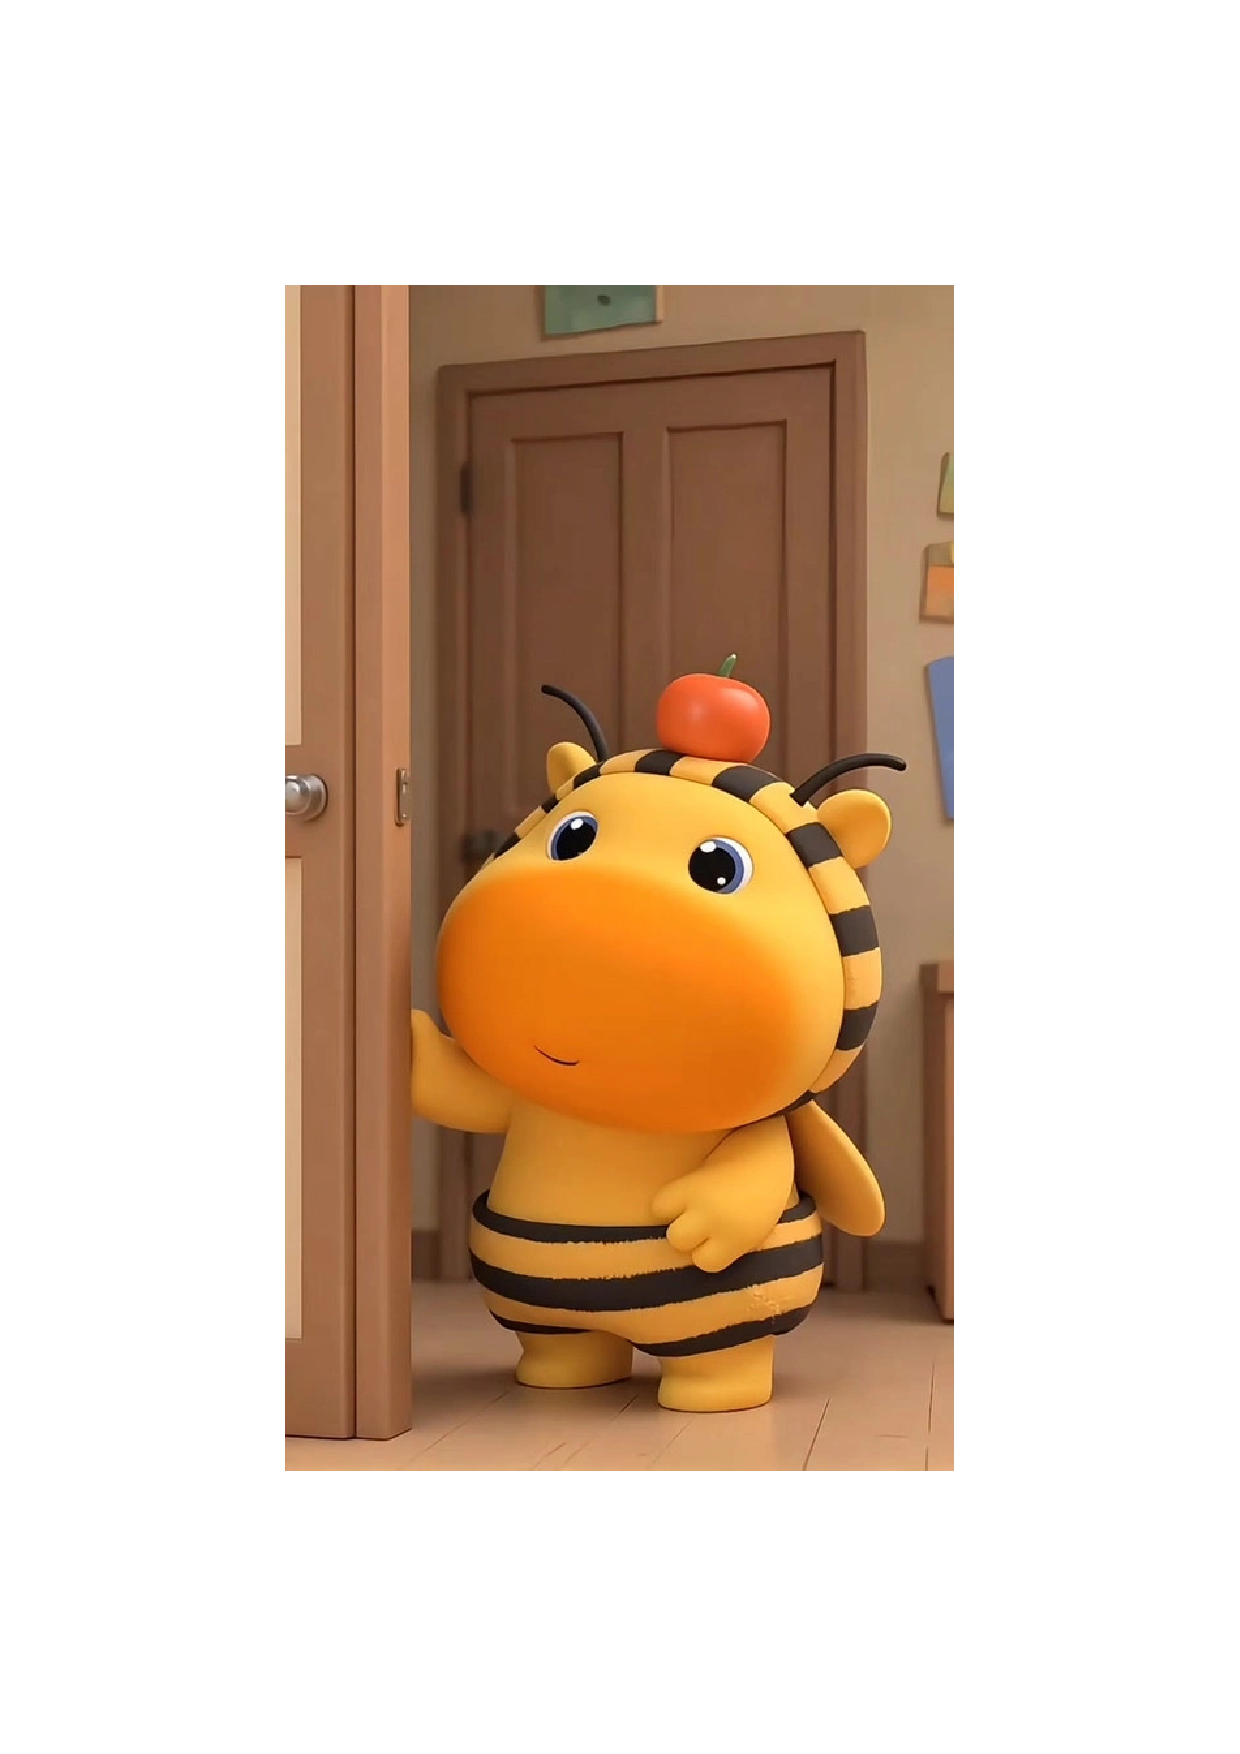
\includegraphics[width=\textwidth]{images/lulu.pdf}
	\caption{噜噜实拍}
	\label{fig:lulu}
\end{figure*}

\begin{table}[htbp]
	\centering
	\caption{赛博水豚养殖策略与效果对比}
	\begin{tabular}{lll}
		\hline
		养殖策略 & 特征描述 & 传播效果（主观） \\
		\hline
		高强度营业型 & 高频更新、情绪波动大 & 容易翻车 \\
		摆烂躺平型   & 低频更新、稳定输出   & 极易出圈 \\
		随缘放养型   & 完全不可预测         & 看命 \\
		\hline
	\end{tabular}
	\label{tab:comparison}
\end{table}
\subsubsection{噜噜}

\subsubsection{奶龙}

\subsubsection{牛牛}


